
%(BEGIN_QUESTION)
% Copyright 2010, Tony R. Kuphaldt, released under the Creative Commons Attribution License (v 1.0)
% This means you may do almost anything with this work of mine, so long as you give me proper credit

Et \textit{Pirani gauge} er et spesielt trykkinstrument laget for å måle svært lave trykk (hardt vakuum).  Det bruker to elektrisk oppvarmede filamenter, hvor det ene er forseglet i et vakuum-``referanse''kammer, mens det andre er eksponert for prosessgass-trykket som måles.  Gassmolekyler som treffer målefilamentet kjøler det ned og reduserer motstanden:

$$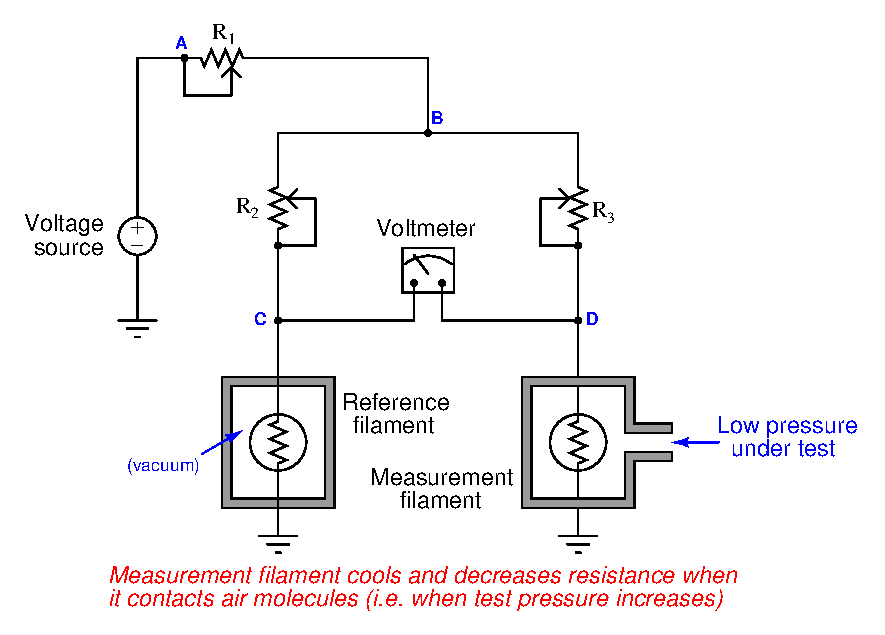
\includegraphics[width=15.5cm]{i00300x01.eps}$$

Dette Pirani-instrumentet har imidlertid et problem.  Det viser høyt trykk hele tiden, uansett vakuumnivå koblet til målecellen.  Et digitalt multimeter koblet mellom testpunkt {\bf D} og jord viser 0 volt.

Vurder sannsynligheten for hver spesifisert feil i kretsen.  Vurder én feil av gangen (ingen samtidige feil), og avgjør om hver feil alene kan forklare {\it alle} målinger og symptomer i kretsen.

% No blank lines allowed between lines of an \halign structure!
% I use comments (%) instead, so that TeX doesn't choke.

$$\vbox{\offinterlineskip
\halign{\strut
\vrule \quad\hfil # \ \hfil & 
\vrule \quad\hfil # \ \hfil & 
\vrule \quad\hfil # \ \hfil \vrule \cr
\noalign{\hrule}
%
% First row
{\bf Feil} & {\bf Mulig} & {\bf Umulig} \cr
%
\noalign{\hrule}
%
% Another row
$R_1$ feilet åpen &  &  \cr
%
\noalign{\hrule}
%
% Another row
$R_1$ feilet kortsluttet &  &  \cr
%
\noalign{\hrule}
%
% Another row
$R_2$ feilet åpen &  &  \cr
%
\noalign{\hrule}
%
% Another row
$R_2$ feilet kortsluttet &  &  \cr
%
\noalign{\hrule}
%
% Another row
$R_3$ feilet åpen &  &  \cr
%
\noalign{\hrule}
%
% Another row
$R_3$ feilet kortsluttet &  &  \cr
%
\noalign{\hrule}
%
% Another row
Referansefilament brent av &  &  \cr
%
\noalign{\hrule}
%
% Another row
Målefilament brent av &  &  \cr
%
\noalign{\hrule}
} % End of \halign 
}$$ % End of \vbox


\underbar{file i00300}
%(END_QUESTION)





%(BEGIN_ANSWER)

% No blank lines allowed between lines of an \halign structure!
% I use comments (%) instead, so that TeX doesn't choke.

$$\vbox{\offinterlineskip
\halign{\strut
\vrule \quad\hfil # \ \hfil & 
\vrule \quad\hfil # \ \hfil & 
\vrule \quad\hfil # \ \hfil \vrule \cr
\noalign{\hrule}
%
% First row
{\bf Feil} & {\bf Mulig} & {\bf Umulig} \cr
%
\noalign{\hrule}
%
% Another row
$R_1$ feilet åpen &  & $\surd$ \cr
%
\noalign{\hrule}
%
% Another row
$R_1$ feilet kortsluttet &  & $\surd$ \cr
%
\noalign{\hrule}
%
% Another row
$R_2$ feilet åpen &  & $\surd$ \cr
%
\noalign{\hrule}
%
% Another row
$R_2$ feilet kortsluttet &  & $\surd$ \cr
%
\noalign{\hrule}
%
% Another row
$R_3$ feilet åpen & $\surd$ &  \cr
%
\noalign{\hrule}
%
% Another row
$R_3$ feilet kortsluttet &  & $\surd$ \cr
%
\noalign{\hrule}
%
% Another row
Referansefilament brent av &  & $\surd$ \cr
%
\noalign{\hrule}
%
% Another row
Målefilament brent av &  & $\surd$ \cr
%
\noalign{\hrule}
} % End of \halign 
}$$ % End of \vbox


%(END_ANSWER)





%(BEGIN_NOTES)

%INDEX% Measurement, pressure: Pirani gauge
%INDEX% Troubleshooting review: electric circuits

%(END_NOTES)
